\section{User Interface}\label{sec:user-interface}

Enten vidt forskellige prototyper eller så flere bud på de forskellige elementer /sider af applicationen.



\subsection{Prototype}



\subsection{Model-View-Controller Pattern}\label{subsec:model-view-controller-pattern}
The model-view-controller, MVC, is arguably one of the most used architectural pattern used for implementing graphical user interfaces and web applications. This pattern fits the projects needs, and can be used to provide a good and logical structure of the project. The Model-View-Controller Pattern is divided into three components:
\begin{description}
\item[Model] the layer that stores the data. 
\item[View] the visual representation of the model. The view is based on the data found in the model.
\item[Controller] the link between the user and the system. The controller allows the users to change view, and manipulate the model's state. 
\end{description}

\figref{fig:mvc-pattern} shows the MVC pattern in context with a user. As seen, the user has the ability to control the system, by the functionality given. With this functionality, the user can manipulate the model and change views, in the way he sees fit. 

\begin{figure}[H]
     \center{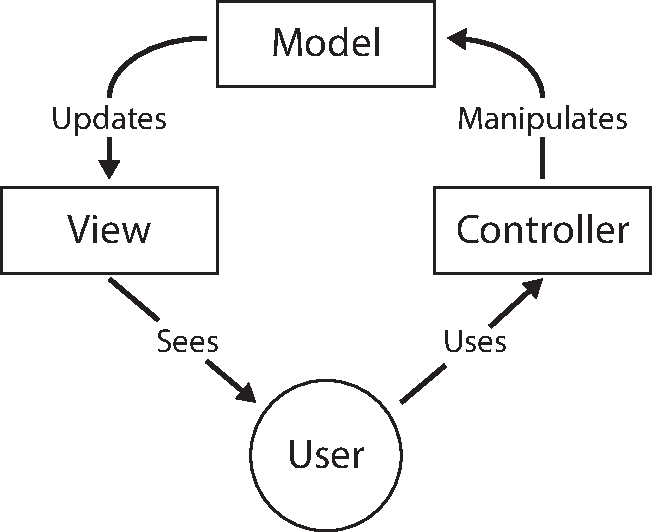
\includegraphics[width=\textwidth -250px]
     {graphics/model-view-controller.pdf}}
     \caption{\label{fig:mvc-pattern} Model-view-controller pattern.}
\end{figure}

Many frameworks that supports the MVC pattern for various languages, such as Django for Python, Rails for Ruby, Maypole for Perl, and so forth, exists.  